\iffalse
\chapter{}

\section{旧约 }
\subsection{亚伯拉罕之约}
%\subsubsection{创世记1课 创造1（Rachael、Joyce），Leo，Stefanie,慧娟，慧洁}
\subsubsection{创世记2课 创造2 Rachael、Joyce，Leo，Stefanie，Luna，Selina，慧娟，}
\subsubsection{创世记3课 犯罪 Rachael、Joyce，Leo，Stefanie，壮壮，Selina，Ethan，Adriana，慧娟，}
\subsubsection{创世记4课 大洪水 Leo，Stefanie，慧娟，慧洁}
\subsubsection{创世记5课 亚伯拉罕 Rachael？，Leo，慧娟，慧洁（15：2-8，没读完）}

\subsection{摩西之约 Leo，Luna，David，Joyce，Rachael}
\subsection{大卫之约 }

\section{新约}
\subsection{耶稣出生}
\subsection{耶稣的受洗}
\subsection{耶稣的神迹}
\subsection{耶稣的教导}
\subsection{耶稣的受死}
\subsection{耶稣的复活}
\subsection{耶稣的再来}
\fi


\chapter{创造 Rachael、Joyce，Leo，Stefanie}
\section{Bible verse}
In the beginning God created the sky and the earth. The earth was empty and had no form. Darkness covered the ocean, and God’s Spirit was moving over the water.

Then God said, “Let there be light!” And there was light. God saw that the light was good. So he divided the light from the darkness. God named the light “day” and the darkness “night.” Evening passed, and morning came. This was the first day.

Then God said, “Let there be something to divide the water in two!” So God made the air to divide the water in two. Some of the water was above the air, and some of the water was below it. God named the air “sky.” Evening passed, and morning came. This was the second day.

Then God said, “Let the water under the sky be gathered together so the dry land will appear.” And it happened. God named the dry land “earth.” He named the water that was gathered together “seas.” God saw that this was good.

Then God said, “Let the earth produce plants. Some plants will make grain for seeds. Others will make fruit with seeds in it. Every seed will produce more of its own kind of plant.” And it happened. The earth produced plants. Some plants had grain for seeds. The trees made fruit with seeds in it. Each seed grew its own kind of plant. God saw that all this was good. Evening passed, and morning came. This was the third day.

Then God said, “Let there be lights in the sky to separate day from night. These lights will be used for signs, seasons, days and years. They will be in the sky to give light to the earth.” And it happened.

So God made the two large lights. He made the brighter light to rule the day. He made the smaller light to rule the night. He also made the stars. God put all these in the sky to shine on the earth. They are to rule over the day and over the night. He put them there to separate the light from the darkness. God saw that all these things were good. Evening passed, and morning came. This was the fourth day.

Then God said, “Let the water be filled with living things. And let birds fly in the air above the earth.”

So God created the large sea animals. He created every living thing that moves in the sea. The sea is filled with these living things. Each one produces more of its own kind. God also made every bird that flies. And each bird produces more of its own kind. God saw that this was good. God blessed them and said, “Have many young ones and grow in number. Fill the water of the seas, and let the birds grow in number on the earth.” Evening passed, and morning came. This was the fifth day.

Then God said, “Let the earth be filled with animals. And let each produce more of its own kind. Let there be tame animals and small crawling animals and wild animals. And let each produce more of its kind.” And it happened.

So God made the wild animals, the tame animals and all the small crawling animals to produce more of their own kind. God saw that this was good.

Then God said, “Let us make human beings in our image and likeness. And let them rule over the fish in the sea and the birds in the sky. Let them rule over the tame animals, over all the earth and over all the small crawling animals on the earth.”

So God created human beings in his image. In the image of God he created them. He created them male and female. God blessed them and said, “Have many children and grow in number. Fill the earth and be its master. Rule over the fish in the sea and over the birds in the sky. Rule over every living thing that moves on the earth.”

God said, “Look, I have given you all the plants that have grain for seeds. And I have given you all the trees whose fruits have seeds in them. They will be food for you. I have given all the green plants to all the animals to eat. They will be food for every wild animal, every bird of the air and every small crawling animal.” And it happened. God looked at everything he had made, and it was very good. Evening passed, and morning came. This was the sixth day.

\newpage
\section{questions of creation}
\subsection{questions 1:1-5}
\begin{itemize}
\item What was created in the 1st day? 
\item Before the 1st day what were already there? 
\item In the 1st day, morning and evening, which appeared first?
\end{itemize}

\subsection{questions 1:6-13}
\begin{itemize}
\item What was created in the 2nd day?
\item What did the air separate?
\item What appeared in the 3rd day?
\end{itemize}

\subsection{questions 1:14-23}
\begin{itemize}
\item What did God created in the 4th day?
\item What did God created in the 5th day?
\end{itemize}


\subsection{questions 1:24-31}
\begin{itemize}
\item What did God created in the 6th day?
\item Human beings were created according to whose image?
\item Select which is human being’s food and which is animals food?
\begin{itemize}
\item A, All the trees whose fruits have seeds in them. 
\item B, All the green plants
\end{itemize}
\end{itemize}

\subsection{discusions}
\begin{itemize}
\item what did you learn about the characters of God?
\item Why human begins were created in the last day?
\end{itemize}

\newpage
\begin{figure}
\centering
     \begin{subfigure}[b]{0.43\textwidth}
         \centering
         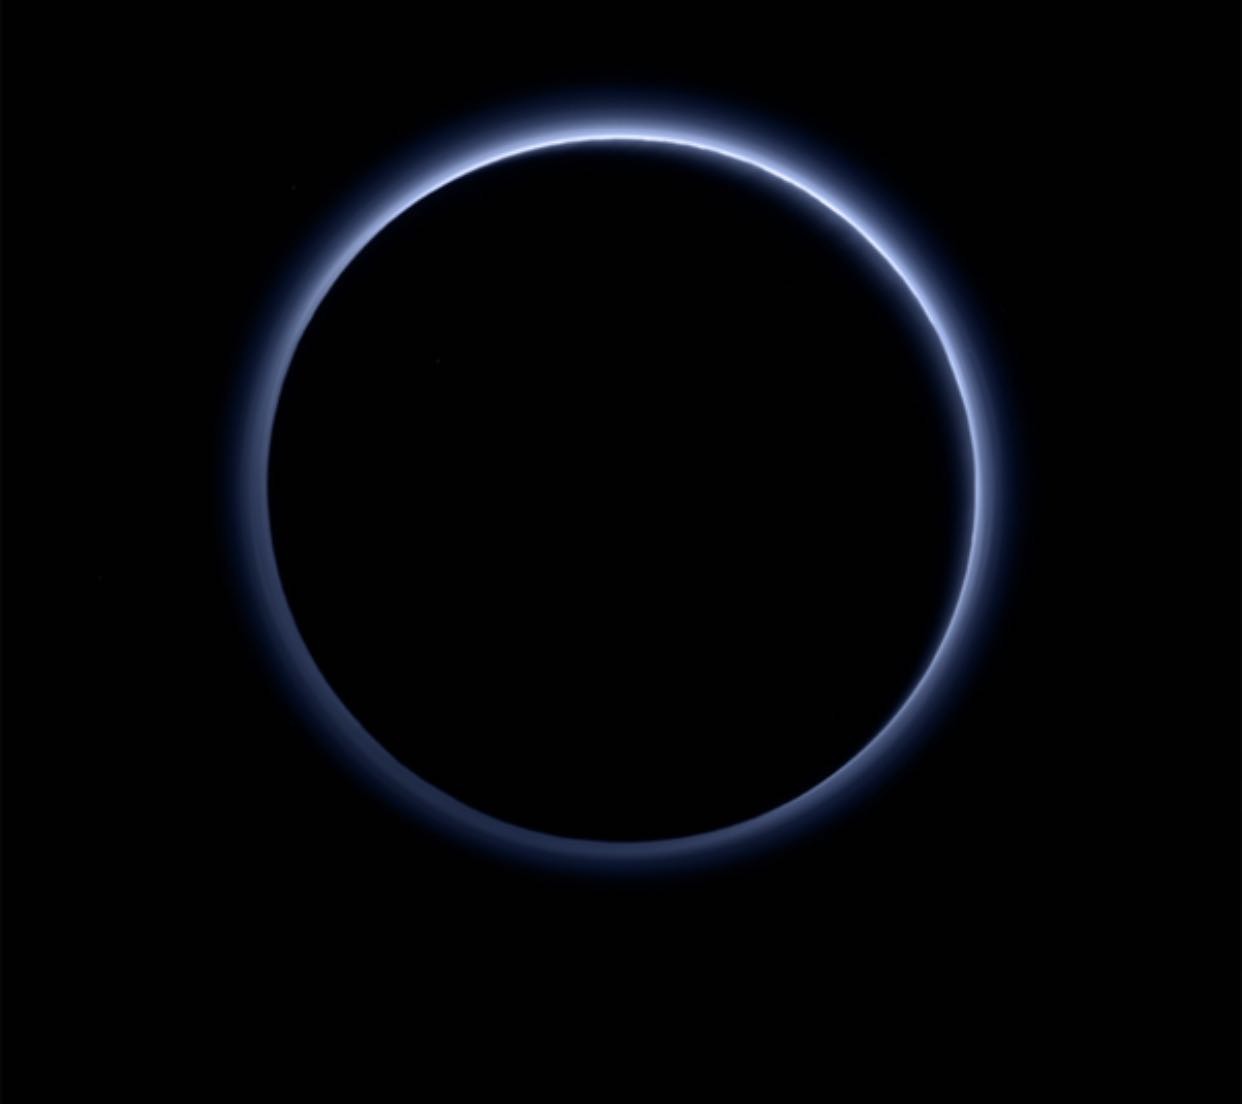
\includegraphics[scale=0.15, ]{ZongJie/bibleChildren/fig/beginning}
\caption{creation of the earth and heaven}
     \end{subfigure}
     \hfill
     \begin{subfigure}[b]{0.5\textwidth}
         \centering
         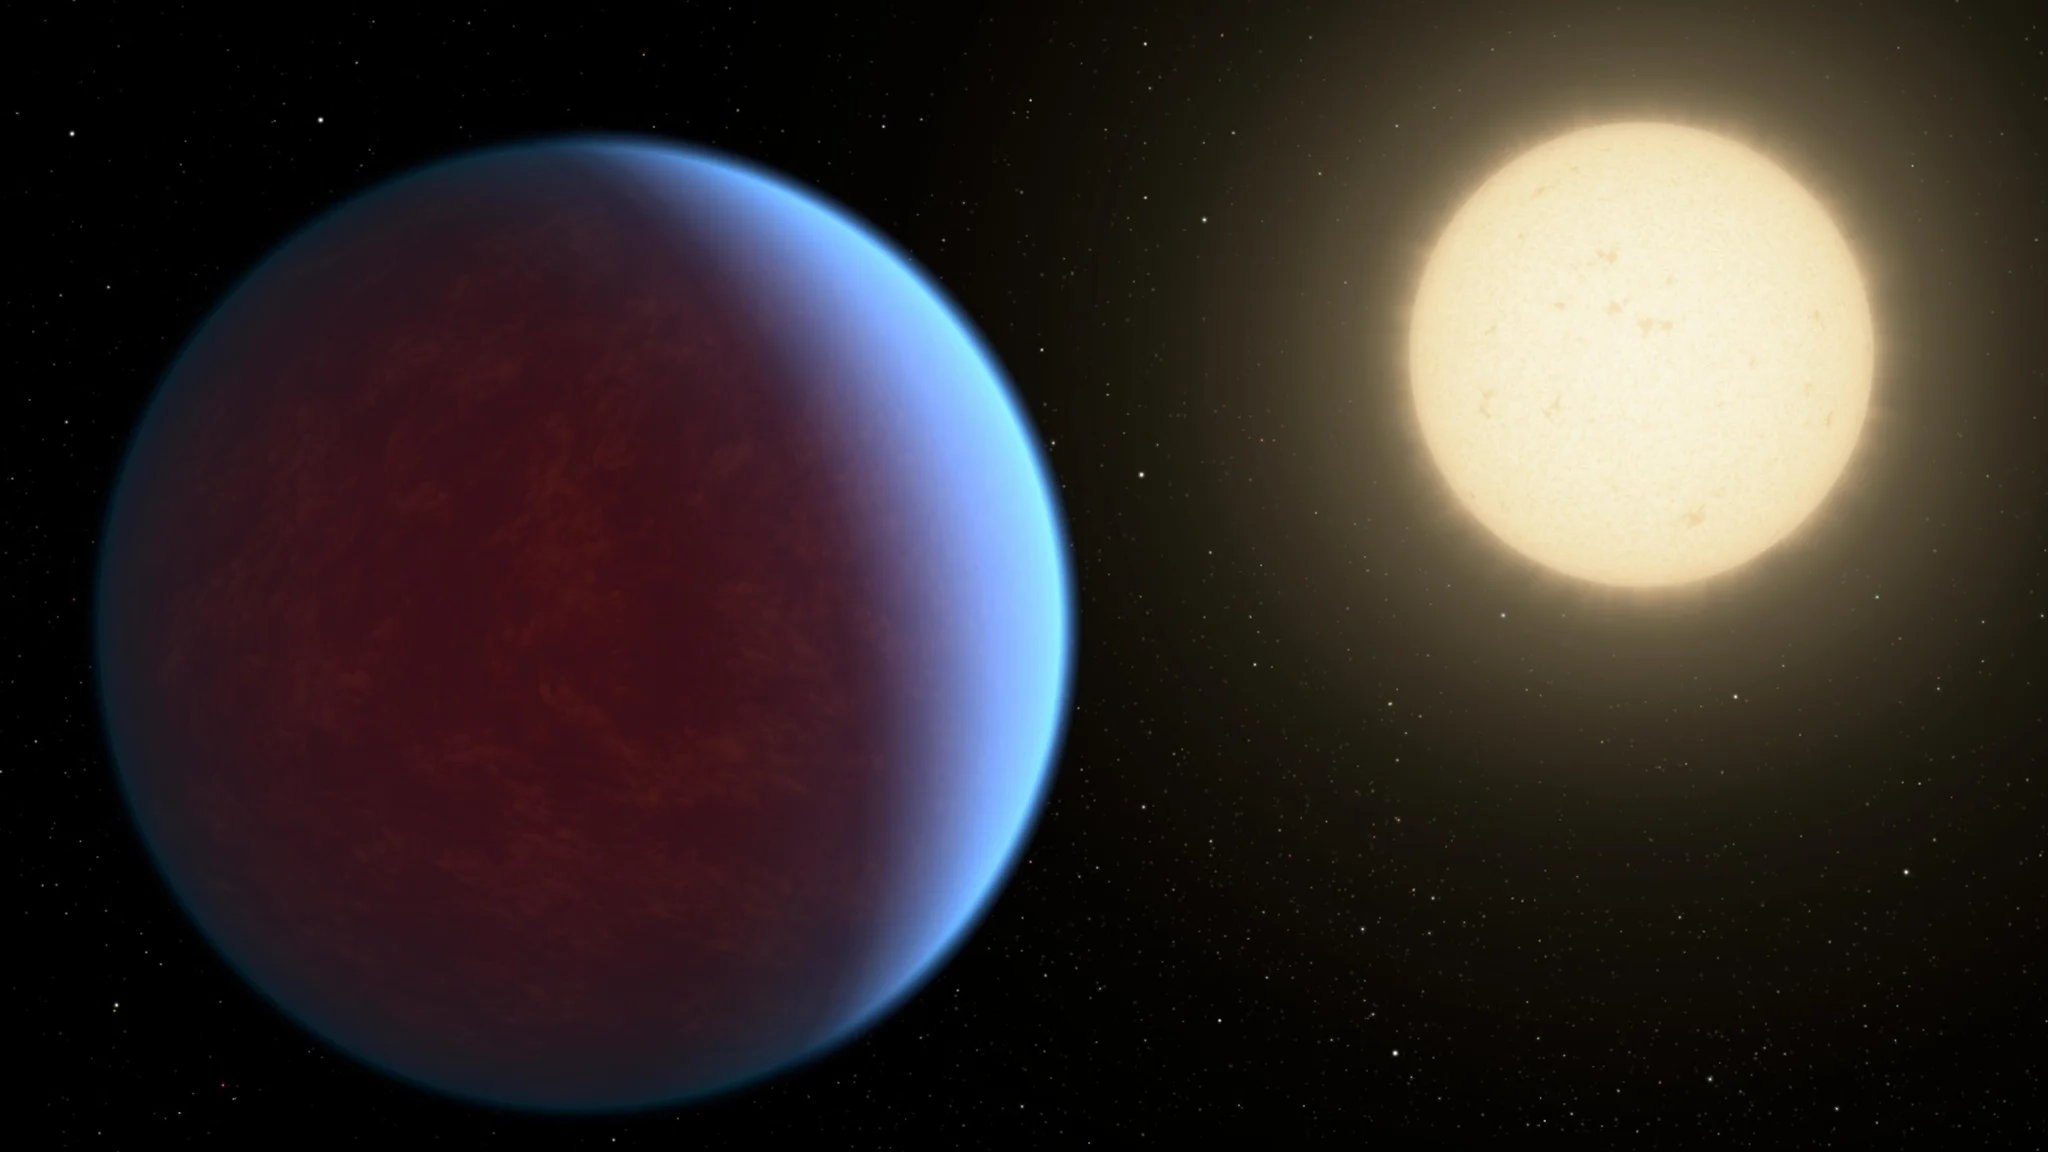
\includegraphics[scale=0.5, ]{ZongJie/bibleChildren/fig/day1}
\caption{creatioin of the light}
     \end{subfigure}
\end{figure}

\begin{figure}
\centering
     \begin{subfigure}[b]{0.3\textwidth}
         \centering
         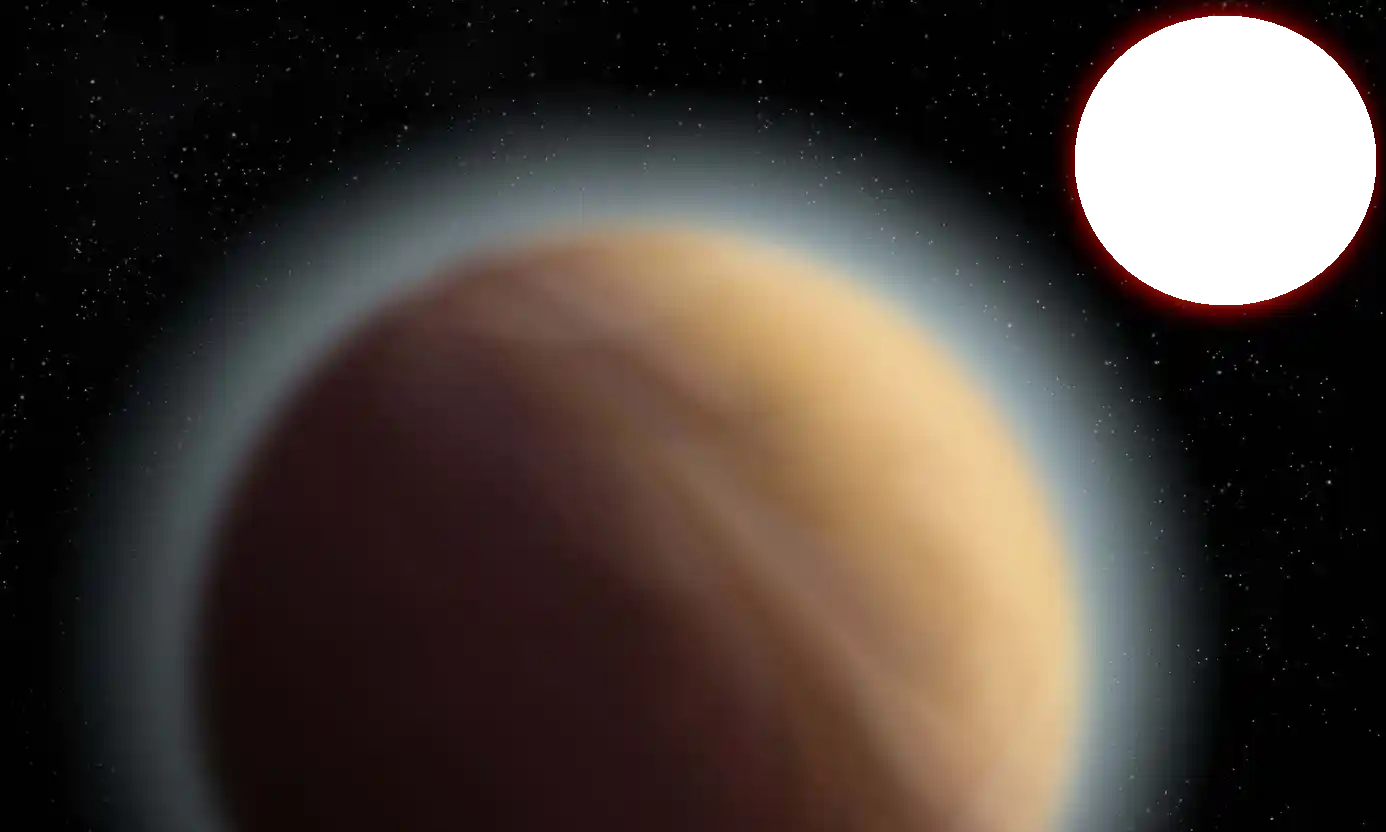
\includegraphics[scale=0.7, ]{ZongJie/bibleChildren/fig/day2}
\caption{creation of the air}
     \end{subfigure}
     \hfill
     \begin{subfigure}[b]{0.3\textwidth}
         \begin{center}
\hspace{-4.cm} 
\vspace{-.75cm}
   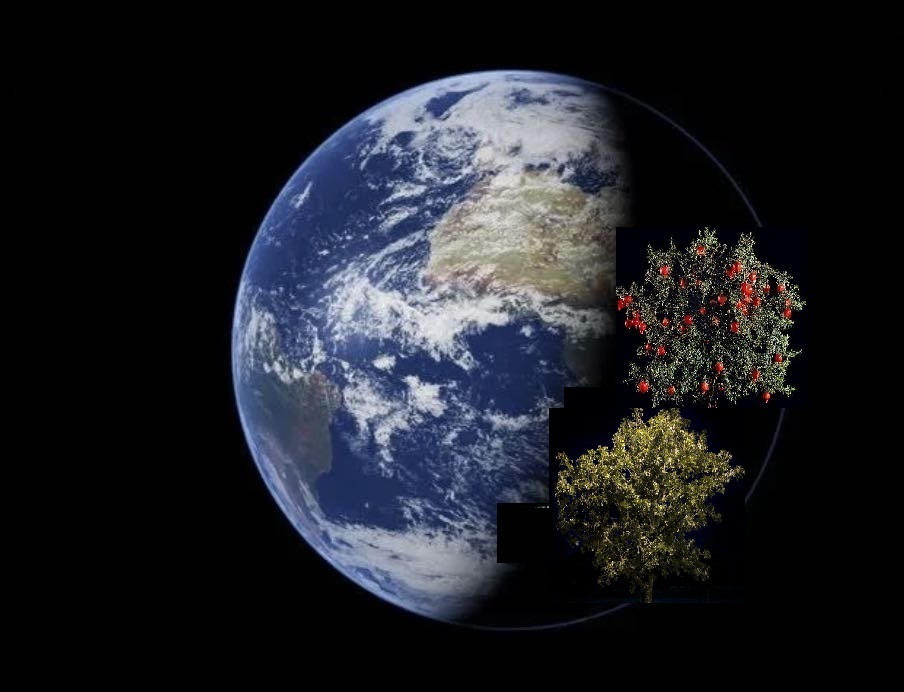
\includegraphics[scale=0.25]{ZongJie/bibleChildren/fig/2thday}
\end{center}
%\vspace{-.25cm}
\caption{creation of the land,sea and fruit trees}
     \end{subfigure}
\end{figure}

\begin{figure}
     \centering
     \begin{subfigure}[b]{0.3\textwidth}
         \centering
         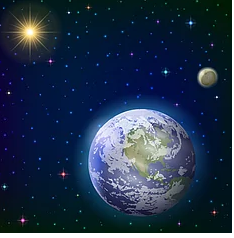
\includegraphics[width=\textwidth]{ZongJie/bibleChildren/fig/star1}
         \caption{creation of sun,moon and stars}
         \label{fig:y equals x}
     \end{subfigure}
     \hfill
     \begin{subfigure}[b]{0.3\textwidth}
         \centering
         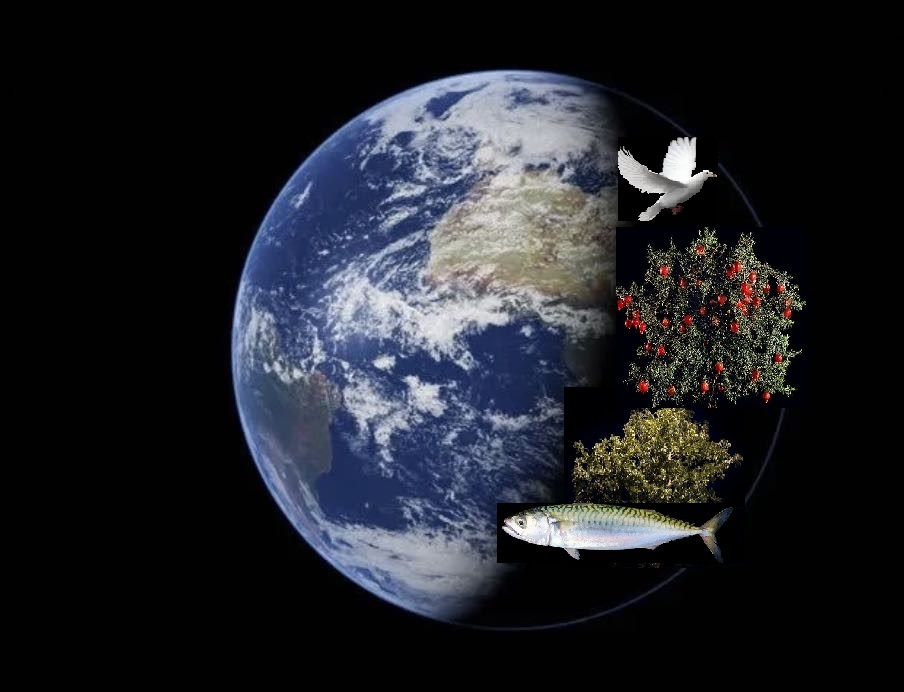
\includegraphics[width=\textwidth]{ZongJie/bibleChildren/fig/2ndday}
         \caption{creation of fish and bird}
         \label{fig:three sin x}
     \end{subfigure}
     \hfill
     \begin{subfigure}[b]{0.3\textwidth}
         \centering
         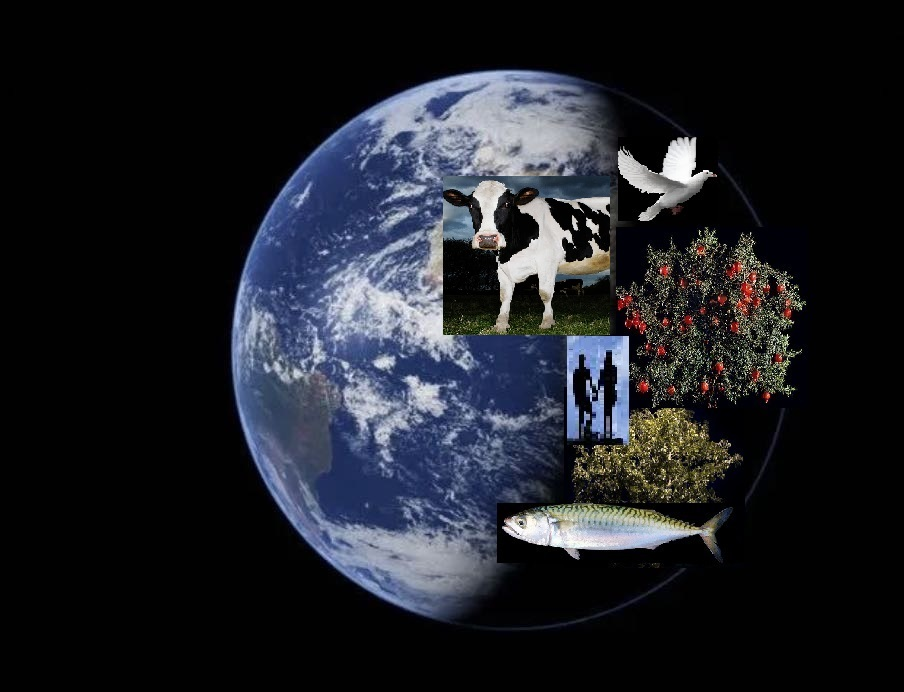
\includegraphics[width=\textwidth]{ZongJie/bibleChildren/fig/6day2}
         \caption{creation of man and woman}
         \label{fig:five over x}
     \end{subfigure}
      %  \caption{Three simple graphs}
     %   \label{fig:three graphs}
\end{figure}






\newpage
\begin{figure}
\centering
     \begin{subfigure}[b]{0.43\textwidth}
         \centering
  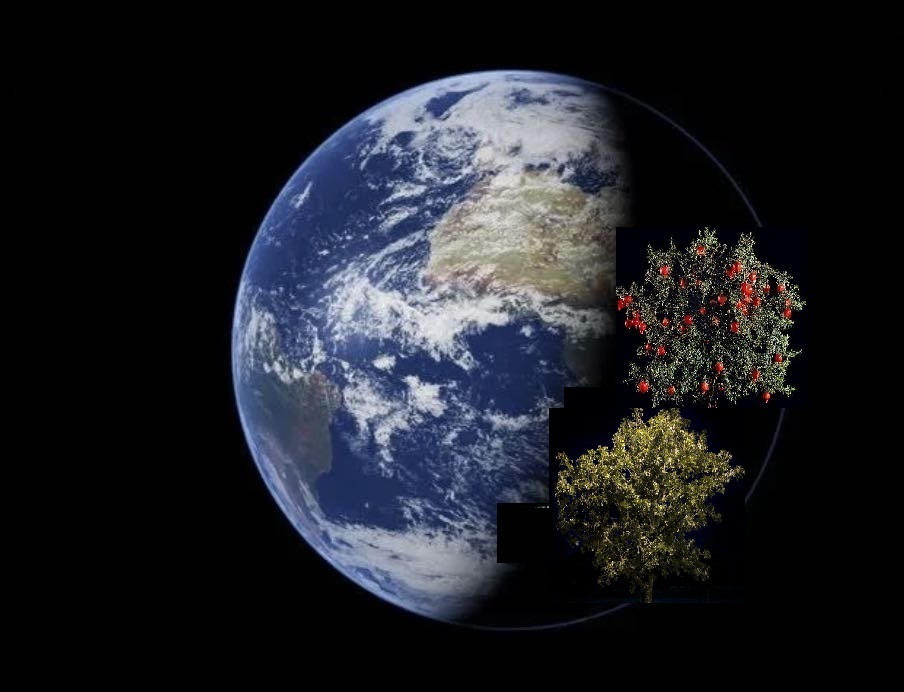
\includegraphics[scale=0.28]{ZongJie/bibleChildren/fig/2thday}       
%\caption{creation of the earth and heaven}
     \end{subfigure}
     \hfill
     \begin{subfigure}[b]{0.43\textwidth}
         \centering
 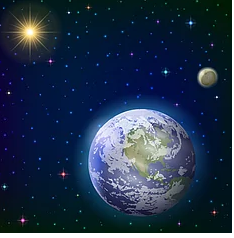
\includegraphics[width=\textwidth]{ZongJie/bibleChildren/fig/star1}
     \end{subfigure}
\end{figure}

\begin{figure}
\centering
     \begin{subfigure}[b]{0.3\textwidth}
         \centering
         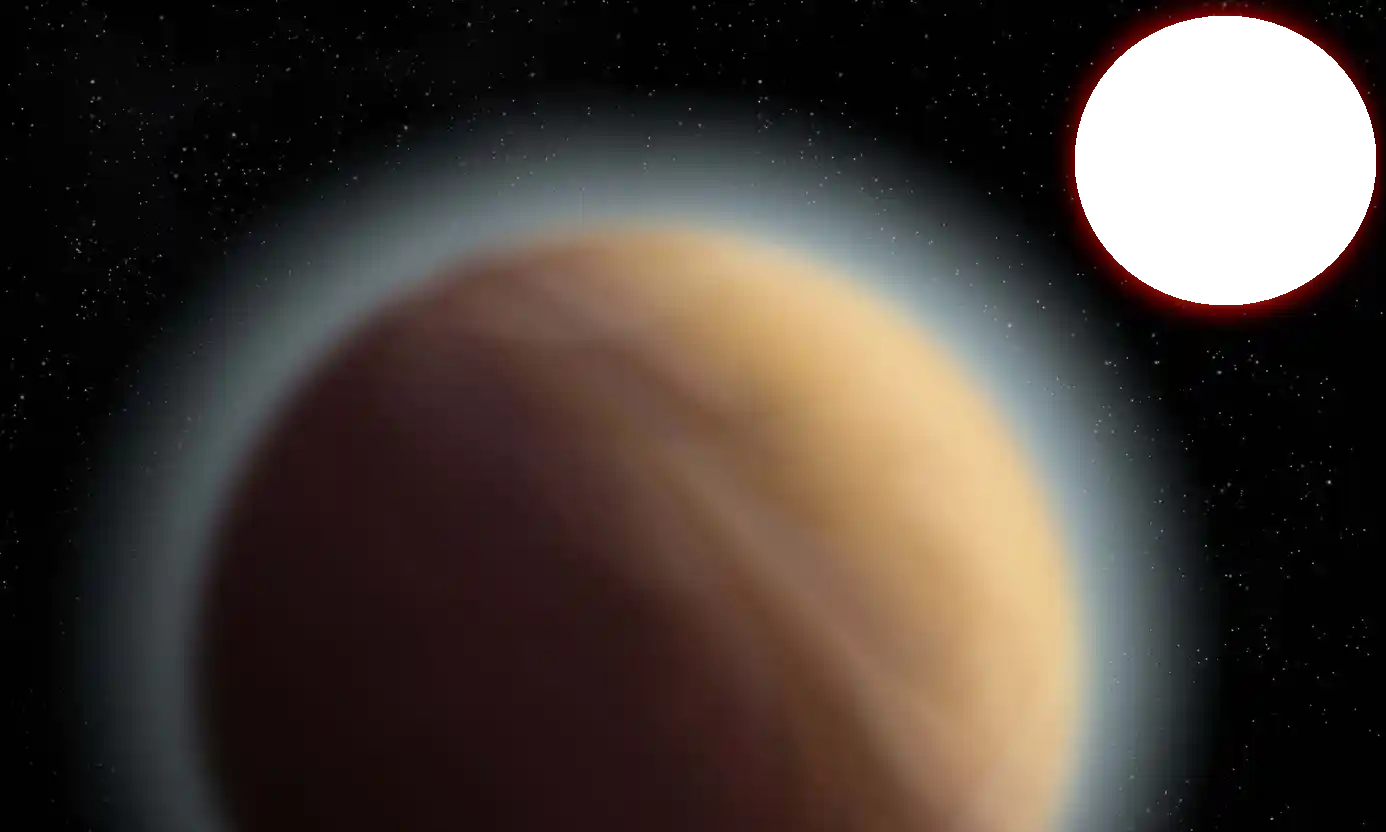
\includegraphics[scale=0.61, ]{ZongJie/bibleChildren/fig/day2}
%\caption{creation of the air}
     \end{subfigure}
     \hfill
     \begin{subfigure}[b]{0.4\textwidth}
         \begin{center}
\hspace{-2.5cm} \vspace{-.65cm}
 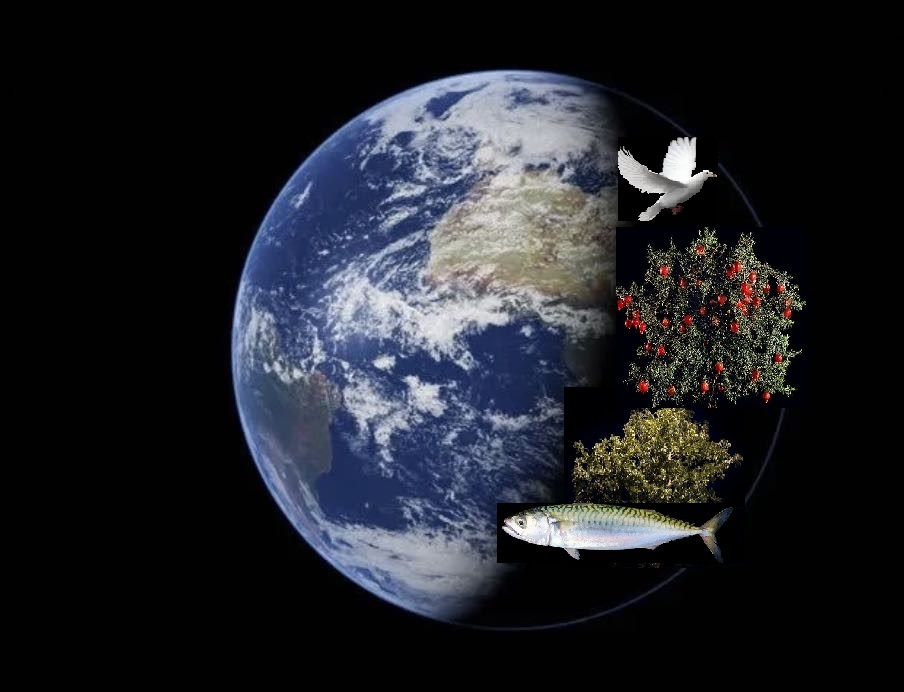
\includegraphics[width=\textwidth]{ZongJie/bibleChildren/fig/2ndday}  
  
\end{center}
     \end{subfigure}
\end{figure}


\begin{figure}
 \centering
\begin{subfigure}[b]{0.3\textwidth}
         \centering
    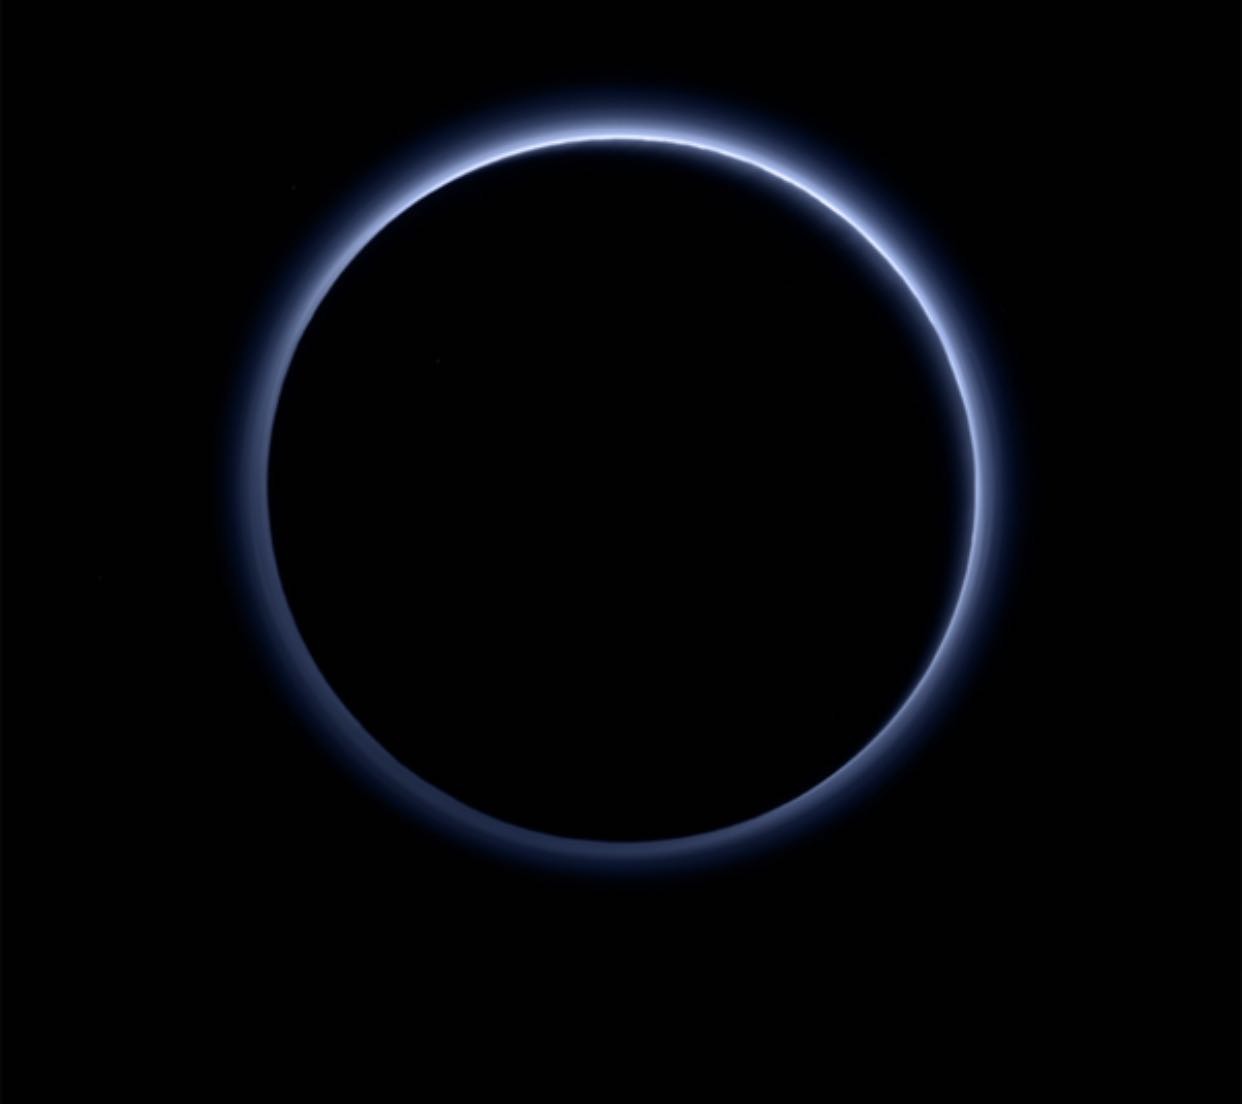
\includegraphics[scale=0.1, ]{ZongJie/bibleChildren/fig/beginning}
     %    \caption{creation of sun,moon and stars}
     %    \label{fig:y equals x}
     \end{subfigure}
     \hfill
     \begin{subfigure}[b]{0.3\textwidth}
         \centering
         
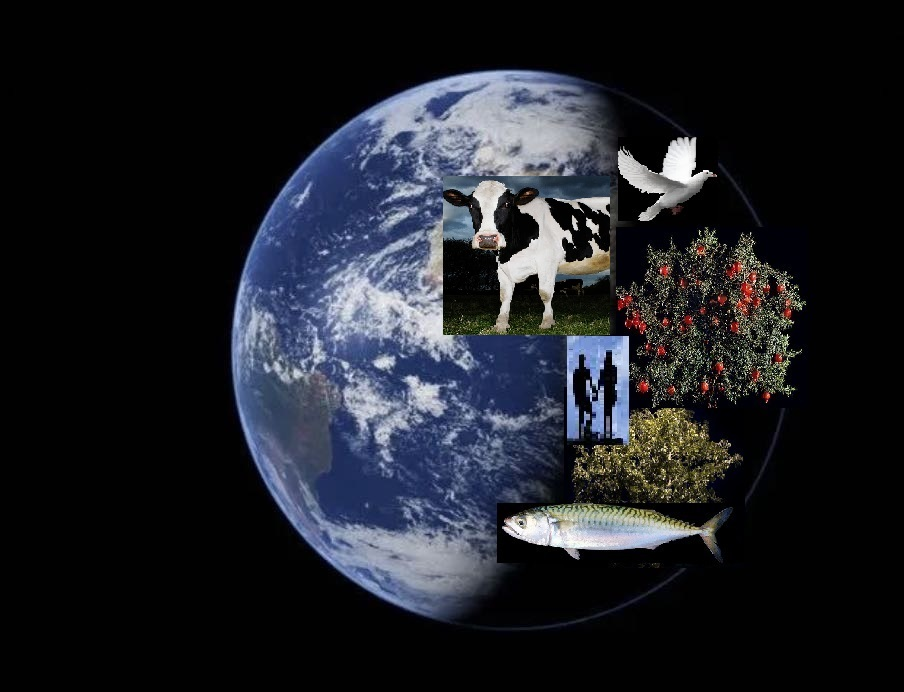
\includegraphics[width=\textwidth]{ZongJie/bibleChildren/fig/6day2}
     \end{subfigure}
     \hfill
     \begin{subfigure}[b]{0.3\textwidth}
         \centering
         
  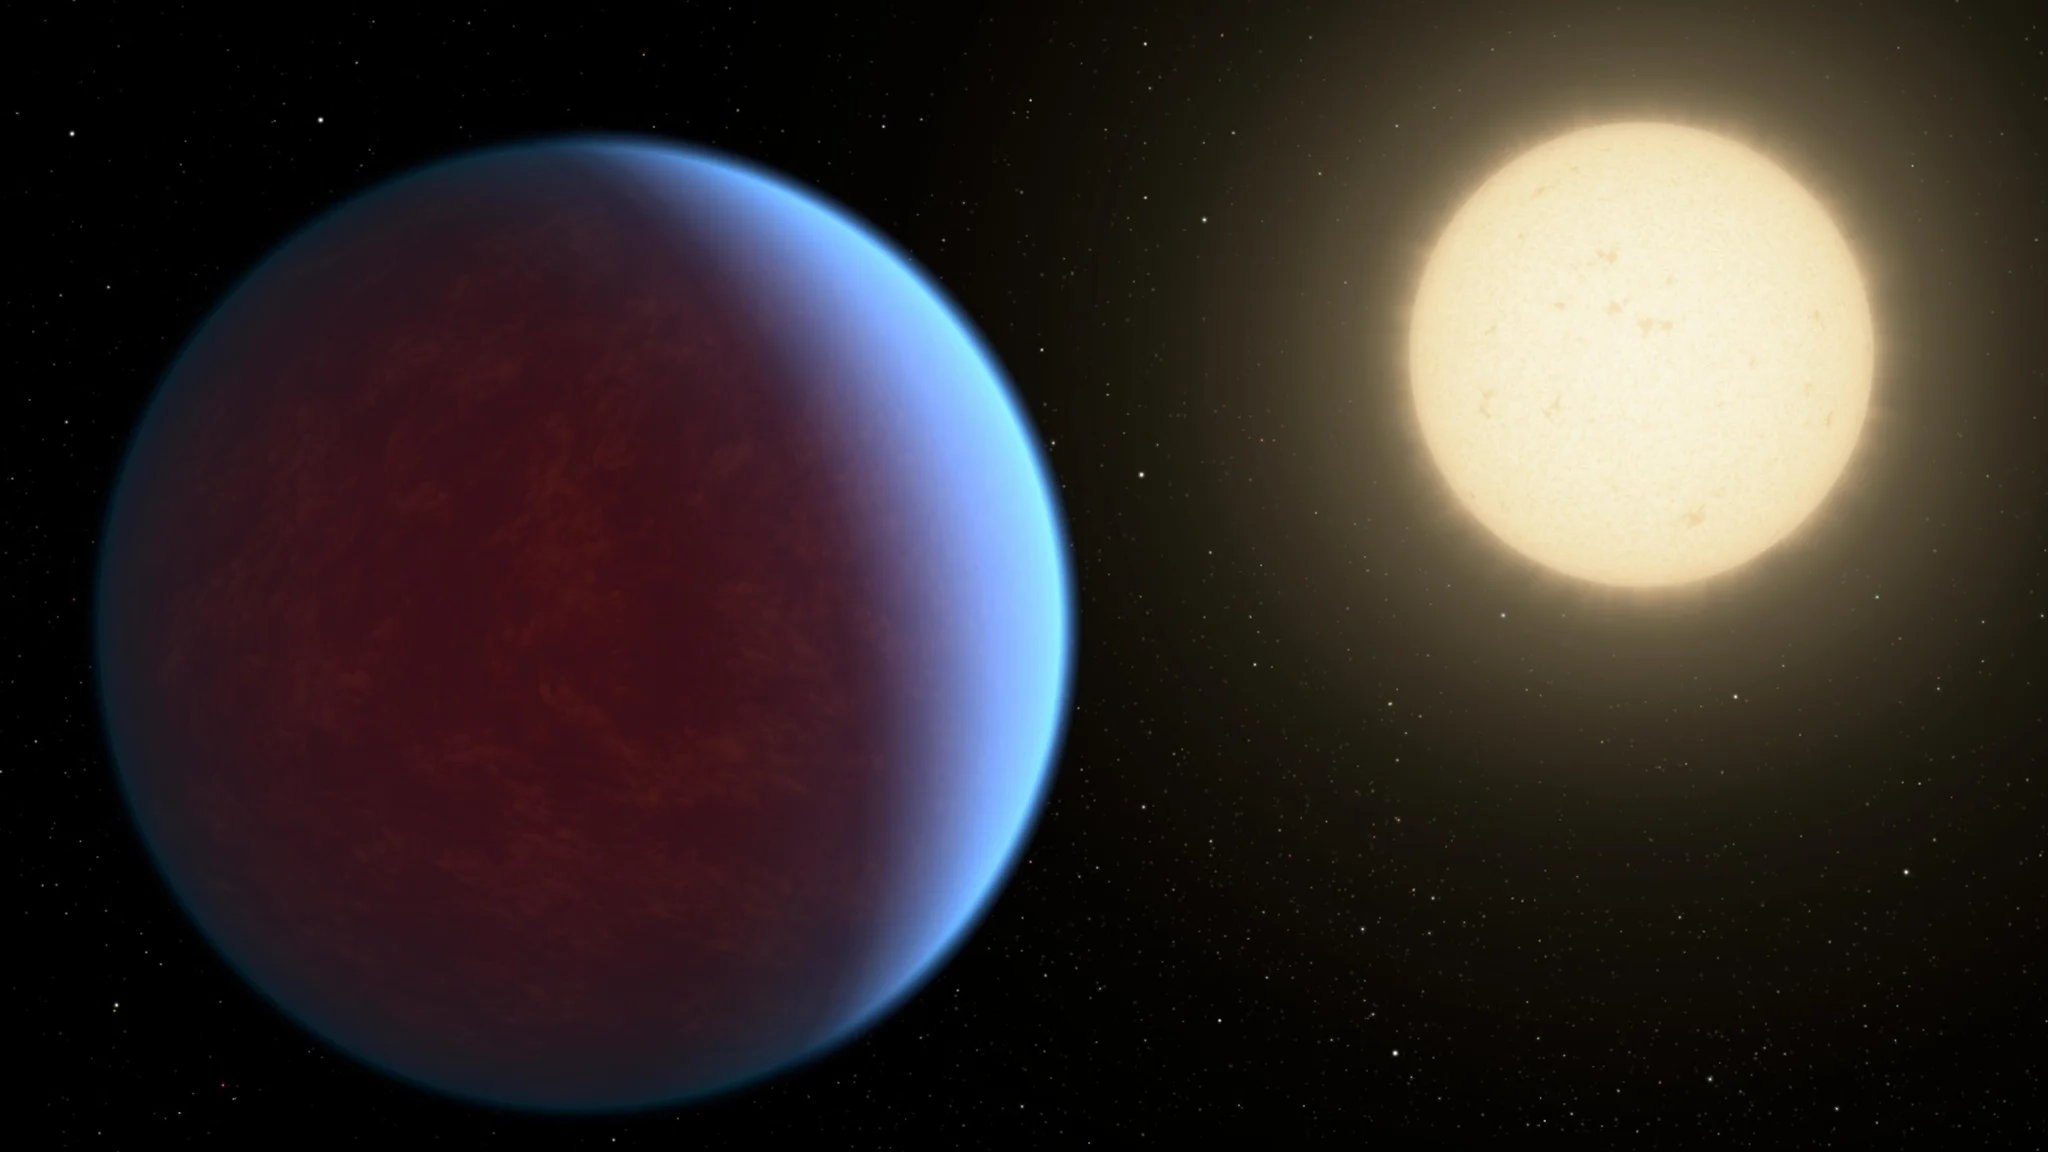
\includegraphics[scale=0.36, ]{ZongJie/bibleChildren/fig/day1}
     \end{subfigure}
  
\end{figure}


\iffalse
\begin{figure}
\centering
     \begin{subfigure}[b]{0.3\textwidth}
         \centering
         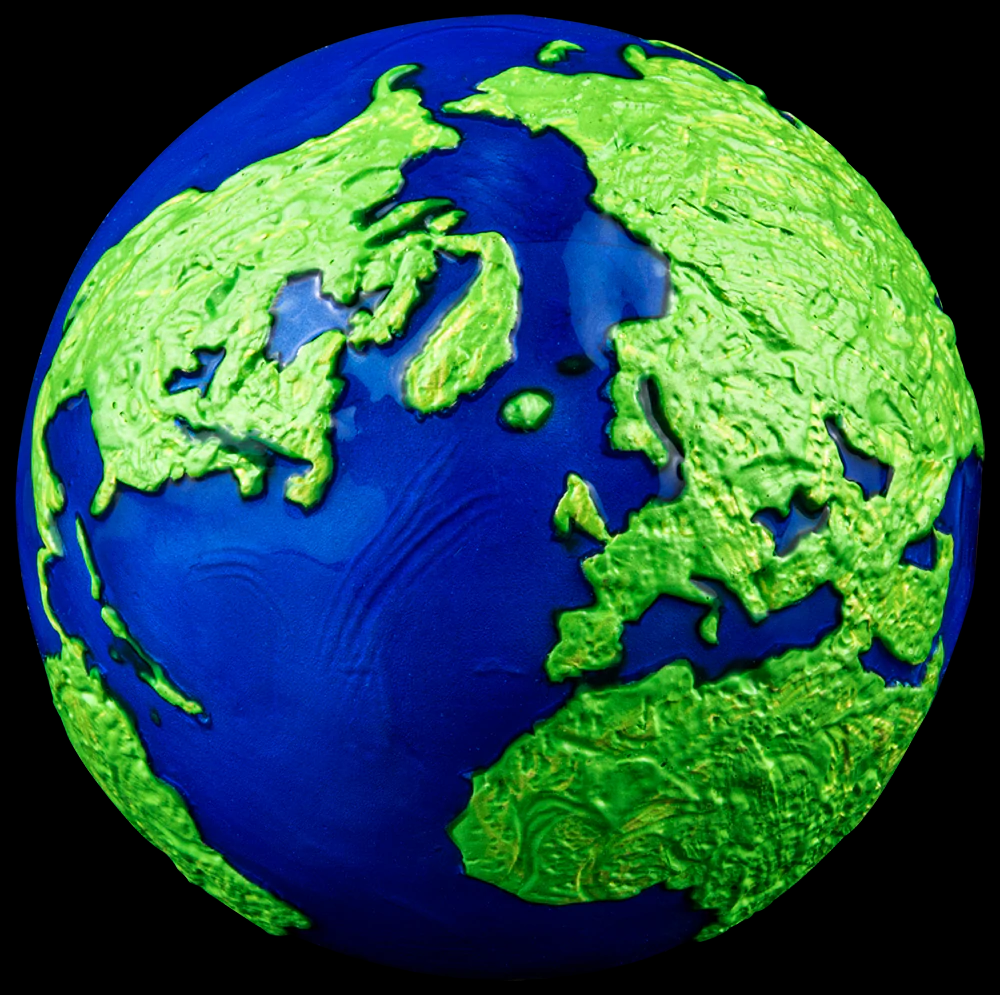
\includegraphics[scale=0.613, ]{ZongJie/bibleChildren/fig/day3}
\caption{day 3: the land and the sea}
     \end{subfigure}
     \hfill
     \begin{subfigure}[b]{0.3\textwidth}
         \centering
         \includegraphics[scale=0.613, ]{ZongJie/bibleChildren/fig/day32}
\caption{day 3: the tree and grass}
     \end{subfigure}
\end{figure}

\begin{figure*}[H]
    \begin{subfigure}[b]{0.35\textwidth}
         \centering
         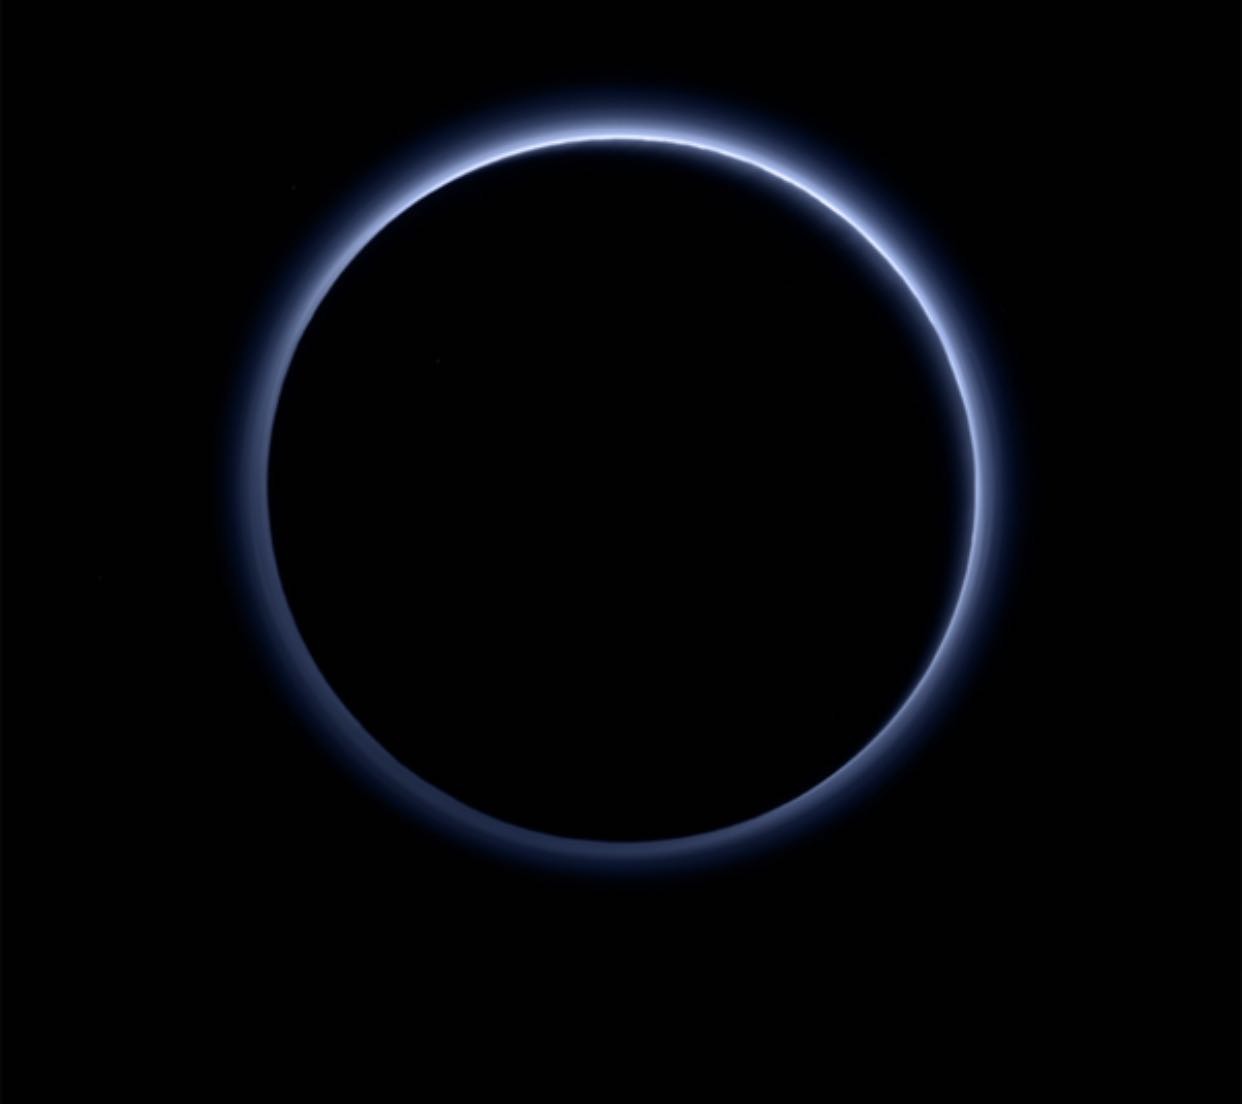
\includegraphics[height=1.86in]{ZongJie/bibleChildren/fig/beginning}
\caption{beginning}
     \end{subfigure}
  ~ 
    \centering
    \begin{subfigure}[b]{0.35\textwidth}
        \centering
        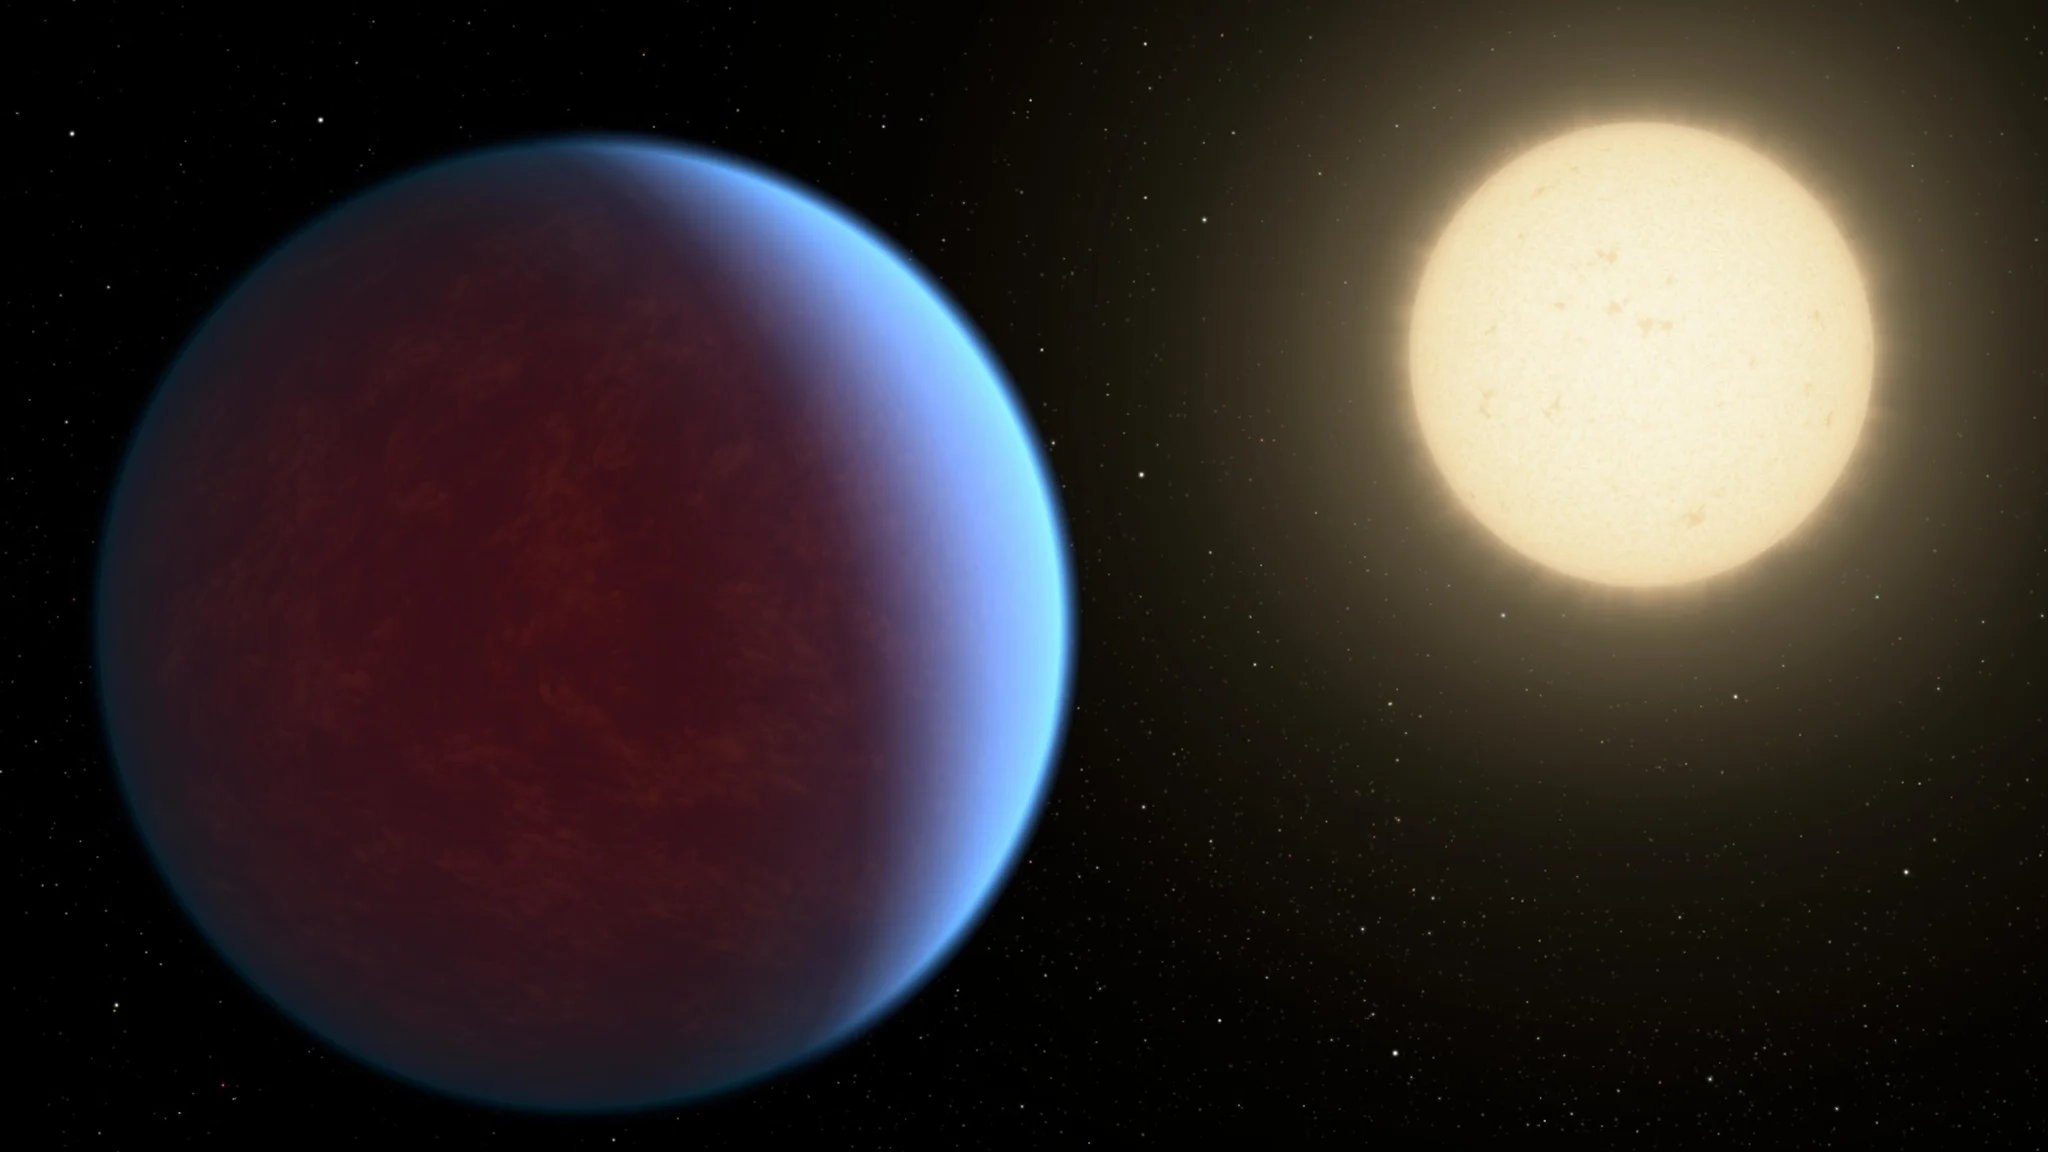
\includegraphics[height=1.86in]{ZongJie/bibleChildren/fig/day1}
        \caption{1st day: light}
    \end{subfigure}%
  ~ 
    \begin{subfigure}[b]{0.35\textwidth}
        \centering
        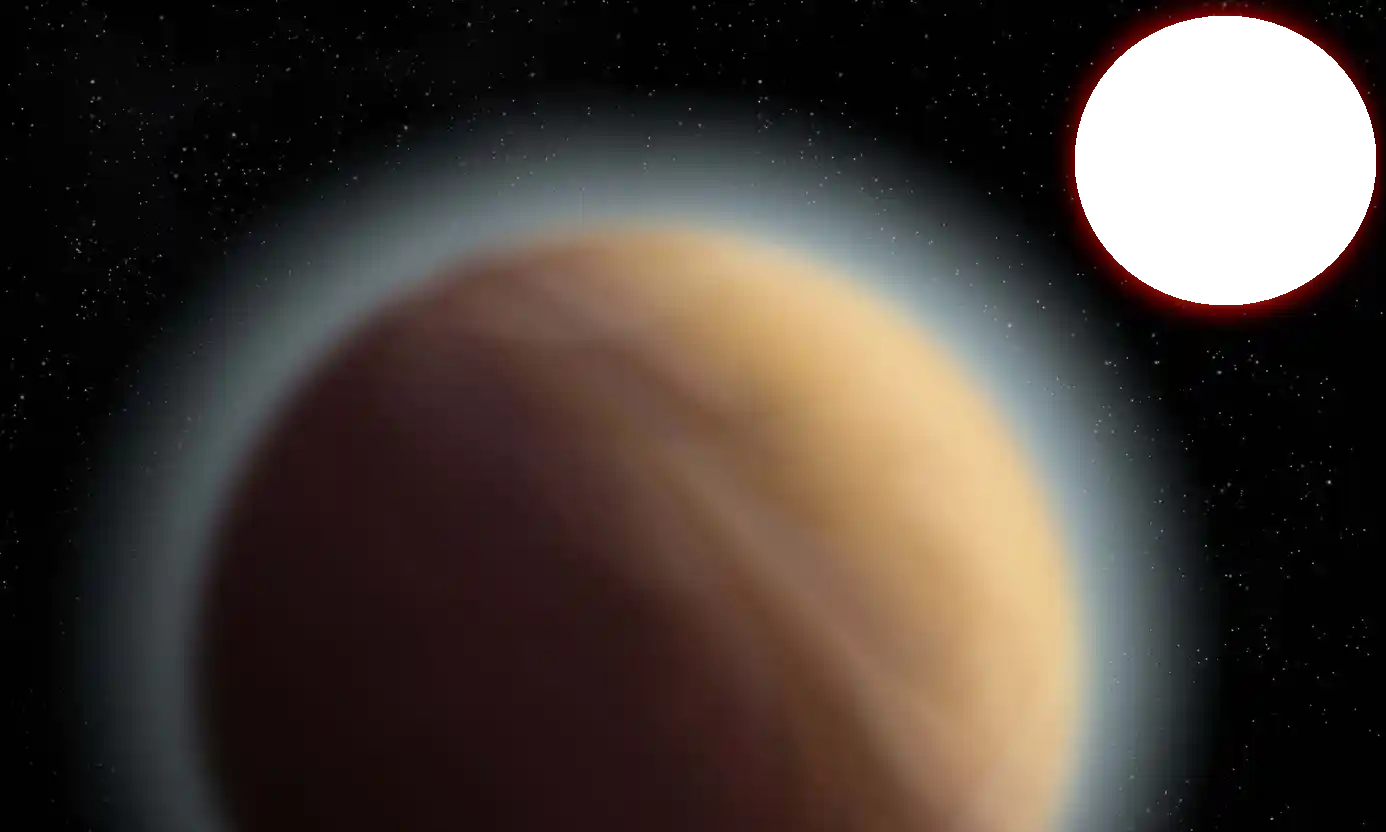
\includegraphics[height=1.86in]{ZongJie/bibleChildren/fig/day2}
      %  \caption{Lorem ipsum, lorem ipsum,Lorem ipsum, lorem ipsum,Lorem ipsum}
    \end{subfigure}
\end{figure*}

\begin{figure*}[H]
    \begin{subfigure}[b]{0.5\textwidth}
         \centering
         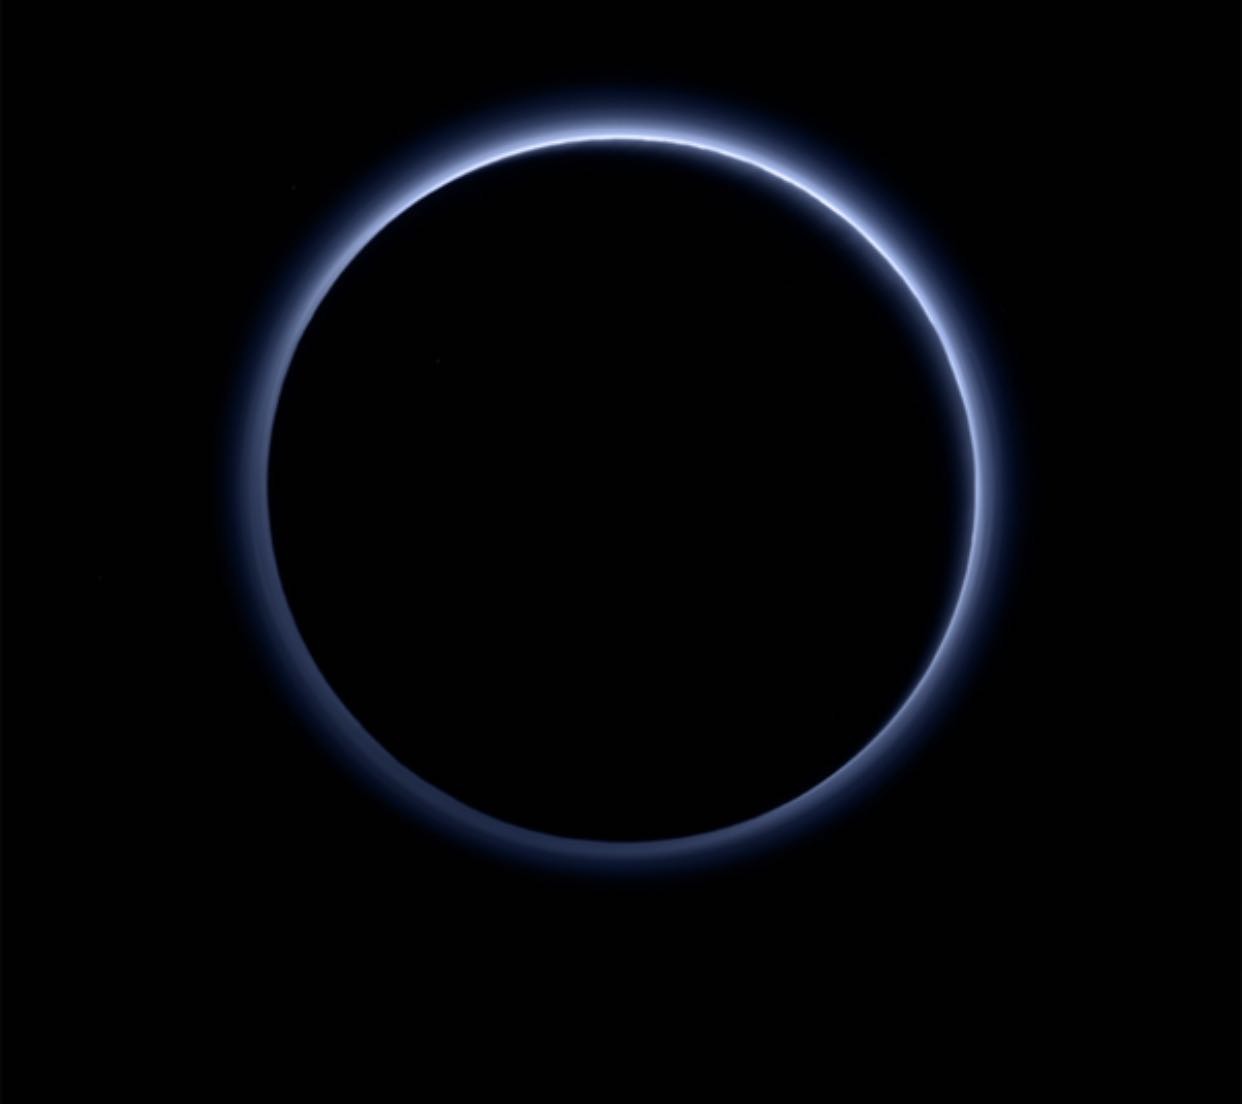
\includegraphics[height=1.86in]{ZongJie/bibleChildren/fig/beginning}
\caption{beginning}
     \end{subfigure}
    ~ 
    \begin{subfigure}[b]{0.5\textwidth}
        \centering
        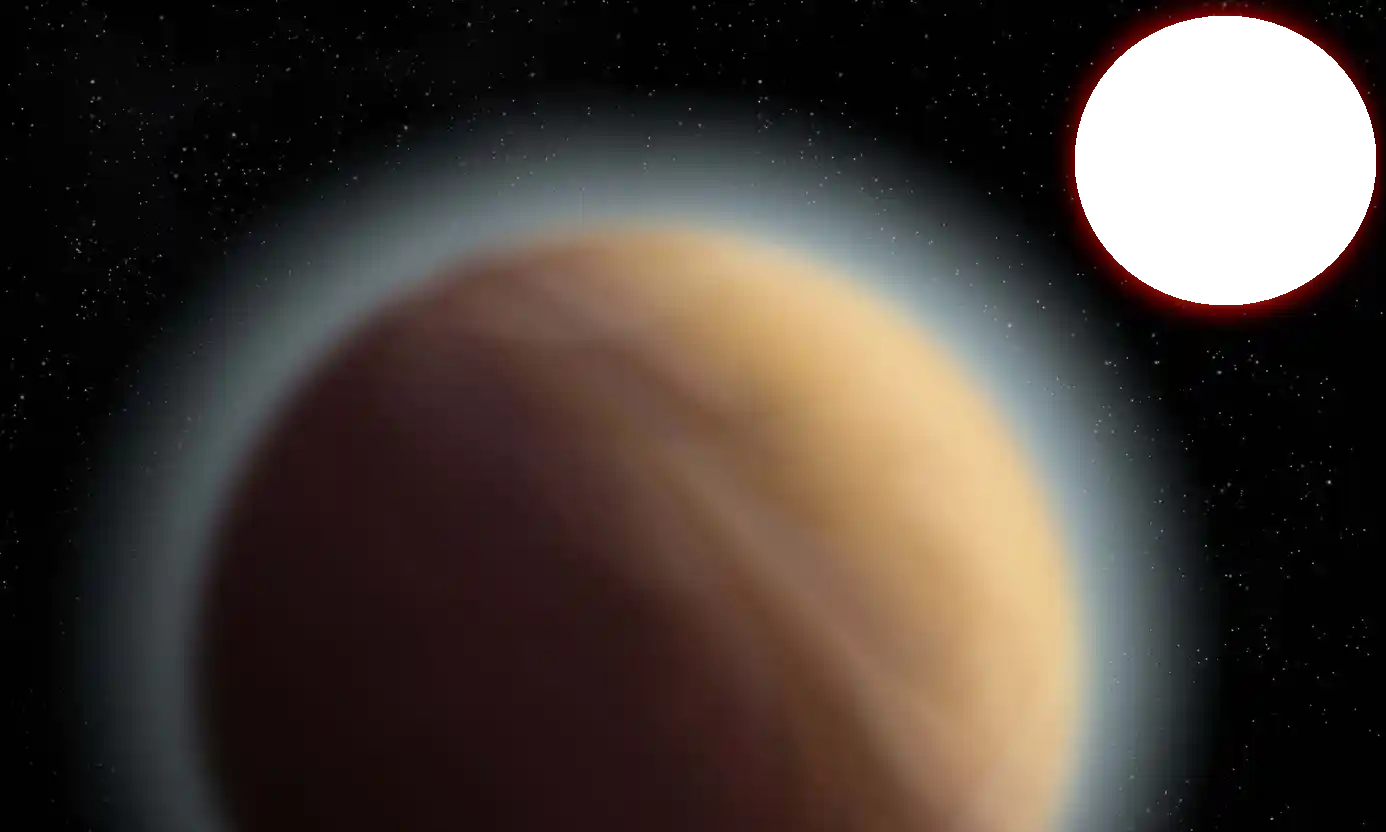
\includegraphics[height=1.86in]{ZongJie/bibleChildren/fig/day2}
      %  \caption{Lorem ipsum, lorem ipsum,Lorem ipsum, lorem ipsum,Lorem ipsum}
    \end{subfigure}
  %  \caption{Caption place holder}
\end{figure*}


https://www.shutterstock.com/image-photo/earth-space-telescope-1261029271
\fi

